\chapter{System Requirement Analysis}


\section{System Requirement Analysis}
1. Redesign the website to make it look modern and attractive.\\
2. Added new feature wherein a store is automatically created once the user register to the Bananoz.\\
3. In this store,Users can upload photographs of the products they purchased from the Bananoz site.\\



%\begin{itemize} 

%\item Generate  the  bill  for  the  user  and  enter  it  in  the  database.
%\item Over the counter charge management.
%\item Preparation of monthly reports.
%\item Status of the parcel.
%\item Built in backup and restore facilities.
%\item hhghfhgh
%\item Trace out the parcel.

%\end{itemize}


\section{Software Process and Development}
The set of general objectives for ”Bananoz Shopping Site” development were defined by the various\\
% This section type your project contents 
\textbf{Agile Methodology}\\

A roadmap is a breakdown of the features that will make up the final product.
This is a crucial component of the planning stage of Agile, because your team will
build these individual features during each sprint..

% This section type your project contents 

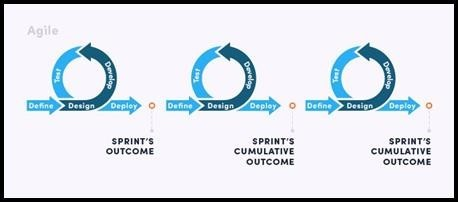
\includegraphics[scale=1.0]{Ch2/agile.jpg}

\label{fig:Prototype Model}

% Diagram change as per your project demands

\section{Scope of Proposed System}
Our experts found that the UI/UX of the old website was outdated and sluggish.During our research, we also found that the overall performance of the old website was slow due to several bugs and errors.\\
In the previous website, users could not add information regarding their personal portfolios and websites.Also, users were unable to share photos and reviews of purchased items on the website.



%\section{Hardware & Software Specifications}


% Write scope of your system.

\section{Technical Specification}
\textbullet \hspace{0.2cm} \textbf{Server}\\
Processor		:	Pentium 3\\
RAM          	: 	Min. 512 MB\\
Hard Disk		: 	Min. 480 MB free\\
\textbullet \hspace{0.2cm} \textbf{Client}\\
Processor   		: 	Pentium 3\\
RAM           	: 	Min. 512 MB\\
Hard Disk		: 	Min. 480 MB free\\
\textbullet \hspace{0.2cm} \textbf{Software Specification}\\
Platform	:  	Windows 10\\
Front End		: 	HTML, JavaScript, CSS.\\
Middle ware		: 	Python\\
Back End			: 	Expess.Js, Node.Js and MS-SQL \\	
Web Browser		: 	Chrome  101.0.4951.67  etc. \\


\subsection{ReactJs Framework}
The top tier of the MERN stack is React.js, the declarative JavaScript framework for creating dynamic client-side applications in HTML. React lets you build up complex interfaces through simple Components, connect them to data on your backend server, and render them as HTML. React is strong suit is handling stateful, data driven interfaces with minimal code and minimal pain, and it has all the bells and whistles you had expected from a modern web framework: great support for forms, error handling, events, lists, and more 
\\

\textbullet \hspace{0.2cm}	It underpins the Model/View/Controller (MVC) approach to web development—a best practice philosophy all developers should adhere to.\\

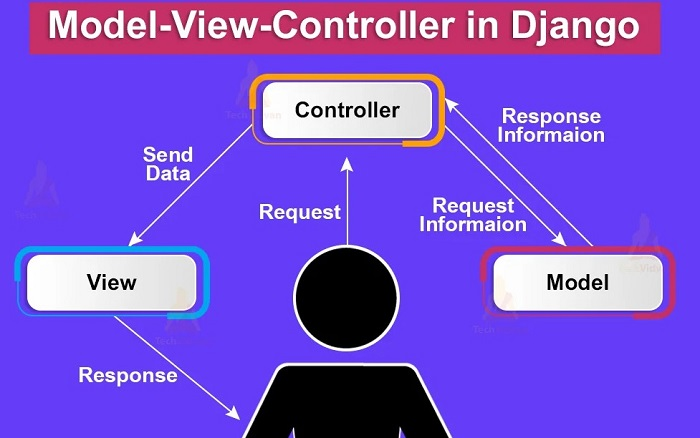
\includegraphics[scale=1.0]{Ch2/mvc1.jpg}


% Diagram change as per your project demands (If required)
\label{fig:MVC Model}

\subsection{Python}
\textbullet \hspace{0.2cm} Python becomes a wonderful choice when it comes to IoT. We can either use it for the backend side of development or the software development of devices. Moreover, Python is available to work on Linux devices, and we can make use of Micro Python for microcontrollers.  \\
\textbullet \hspace{0.2cm} Python is the coding language that we can use to reduce the volume of data that we need to deal with, accessible in the cloud. Python recognizes the needs regardless of whether we create the IoT project from scratch or interact with actuators, sensors, and accessories. \\  
\textbullet \hspace{0.2cm} Some of the many benefits of working with Python for IoT devices are a large number of libraries for all types of platforms and the speed it offers at which we can develop the code. 


%\textbullet \hspace{0.2cm}It’s built on a linear, easy-to-use folder structure.\\


% This section type your project contents 